\documentclass[12pt,a4paper]{article}
\usepackage[utf8]{inputenc}
\usepackage[UTF8]{ctex}
\usepackage{amsmath,amssymb,amsfonts}
\usepackage{graphicx}
\usepackage{float}
\usepackage{booktabs}
\usepackage{caption}
\usepackage{subcaption}
\usepackage{geometry}
\usepackage{hyperref}
\usepackage{enumitem}
\usepackage{listings}
\usepackage{xcolor}

\geometry{left=2.5cm,right=2.5cm,top=2.5cm,bottom=2.5cm}

\title{奇异值分解(SVD)的几何意义与图像压缩应用研究}
\author{研究报告}
\date{\today}

\begin{document}

\maketitle

\begin{abstract}
本文深入研究奇异值分解（Singular Value Decomposition, SVD）的理论基础及其在图像压缩中的应用。首先，从线性代数的角度阐述SVD定理 $A = U\Sigma V^T$ 的数学原理；其次，通过几何视角解析SVD的物理意义——任意线性变换可分解为旋转、缩放和旋转三个步骤；最后，以 $32 \times 32$ 灰度图像为实验对象，通过保留不同数量的奇异值实现图像压缩，并对压缩效果进行定量分析。实验结果表明，仅保留前 $k$ 个奇异值即可在压缩比和图像质量之间取得良好平衡，验证了SVD在图像压缩领域的有效性。

\textbf{关键词：} 奇异值分解；图像压缩；线性变换；几何意义；矩阵分解
\end{abstract}

\newpage
\tableofcontents
\newpage

\section{引言}

\subsection{研究背景}

在数字图像处理领域，图像压缩是一项关键技术。随着多媒体数据的爆炸式增长，高效的图像压缩算法对于存储和传输至关重要。奇异值分解（SVD）作为线性代数中最重要的矩阵分解方法之一，在数据压缩、降维、噪声消除等领域有着广泛的应用。

\subsection{研究目的}

本文旨在：
\begin{enumerate}[label=(\arabic*)]
    \item 阐释SVD定理的数学原理与推导过程
    \item 从几何角度深入理解SVD的物理意义
    \item 通过实验验证SVD在图像压缩中的有效性
    \item 分析压缩参数对图像质量的影响
\end{enumerate}

\subsection{论文结构}

本文共分为六章：第一章为引言；第二章介绍SVD的理论基础；第三章阐述SVD的几何意义；第四章描述图像压缩的实现方法；第五章展示实验结果并进行分析；第六章总结全文并展望未来研究方向。

\section{SVD理论基础}

\subsection{奇异值分解定理}

对于任意实数矩阵 $A \in \mathbb{R}^{m \times n}$，其奇异值分解定义为：

\begin{equation}
    A = U\Sigma V^T
\end{equation}

其中：
\begin{itemize}
    \item $U \in \mathbb{R}^{m \times m}$ 是正交矩阵，其列向量称为左奇异向量
    \item $\Sigma \in \mathbb{R}^{m \times n}$ 是对角矩阵，对角线元素 $\sigma_1 \geq \sigma_2 \geq \cdots \geq \sigma_r > 0$ 称为奇异值
    \item $V \in \mathbb{R}^{n \times n}$ 是正交矩阵，其列向量称为右奇异向量
    \item $r = \text{rank}(A)$ 是矩阵 $A$ 的秩
\end{itemize}

\subsection{奇异值的性质}

奇异值具有以下重要性质：

\begin{enumerate}[label=(\arabic*)]
    \item \textbf{非负性：} 所有奇异值均为非负实数，即 $\sigma_i \geq 0$
    \item \textbf{有序性：} 奇异值按降序排列，$\sigma_1 \geq \sigma_2 \geq \cdots \geq \sigma_r$
    \item \textbf{唯一性：} 奇异值是唯一的（但奇异向量可能不唯一）
    \item \textbf{与特征值的关系：} 奇异值 $\sigma_i$ 是矩阵 $A^TA$ 特征值的平方根
\end{enumerate}

\subsection{SVD的计算}

SVD的计算通常通过以下步骤实现：

\begin{enumerate}
    \item 计算 $A^TA$ 的特征值和特征向量
    \item 将特征值按降序排列，奇异值 $\sigma_i = \sqrt{\lambda_i}$
    \item 计算右奇异向量 $V$
    \item 计算左奇异向量 $U = AV\Sigma^{-1}$
\end{enumerate}

在实际应用中，通常使用数值线性代数库（如NumPy的\texttt{numpy.linalg.svd}）进行计算。

\section{SVD的几何意义}

\subsection{线性变换的分解}

SVD的核心几何意义在于：任意线性变换都可以分解为三个基本变换的复合：

\begin{equation}
    A = U \cdot \Sigma \cdot V^T
\end{equation}

这三个变换分别对应：
\begin{enumerate}
    \item \textbf{第一次旋转} ($V^T$)：在输入空间中进行坐标旋转
    \item \textbf{缩放变换} ($\Sigma$)：沿坐标轴方向进行缩放
    \item \textbf{第二次旋转} ($U$)：在输出空间中进行坐标旋转
\end{enumerate}

\subsection{几何解释}

设 $\mathbf{x}$ 为输入向量，则线性变换 $A\mathbf{x}$ 的几何过程为：

\begin{equation}
    A\mathbf{x} = U(\Sigma(V^T\mathbf{x}))
\end{equation}

\begin{enumerate}
    \item $V^T\mathbf{x}$：将输入向量旋转到以右奇异向量为基的坐标系中
    \item $\Sigma(V^T\mathbf{x})$：沿各坐标轴方向进行缩放，缩放因子为对应的奇异值
    \item $U(\Sigma(V^T\mathbf{x}))$：将缩放后的向量旋转到输出空间的坐标系中
\end{enumerate}

\subsection{单位圆的变换}

考虑二维情况下，单位圆在矩阵 $A$ 作用下的变换：

\begin{enumerate}
    \item 原始单位圆
    \item 经过 $V^T$ 旋转后，仍为单位圆（正交变换保持长度）
    \item 经过 $\Sigma$ 缩放后，变为椭圆，椭圆的半轴长度为奇异值
    \item 经过 $U$ 旋转后，椭圆方向改变，但形状不变
\end{enumerate}

这一几何直观解释了为什么奇异值能够捕捉矩阵的"主要成分"——它们决定了变换后椭圆的形状。

\section{SVD图像压缩方法}

\subsection{图像的矩阵表示}

灰度图像可以表示为一个二维矩阵 $A \in \mathbb{R}^{m \times n}$，其中：
\begin{itemize}
    \item $m$ 为图像的高度（像素行数）
    \item $n$ 为图像的宽度（像素列数）
    \item 矩阵元素 $a_{ij}$ 表示像素 $(i,j)$ 的灰度值（通常为0-255）
\end{itemize}

\subsection{SVD压缩原理}

对图像矩阵 $A$ 进行SVD分解：

\begin{equation}
    A = U\Sigma V^T = \sum_{i=1}^{r} \sigma_i \mathbf{u}_i \mathbf{v}_i^T
\end{equation}

其中 $\mathbf{u}_i$ 和 $\mathbf{v}_i$ 分别是 $U$ 和 $V$ 的第 $i$ 列。

压缩的核心思想是保留前 $k$ 个最大的奇异值及其对应的奇异向量，忽略较小的奇异值：

\begin{equation}
    A_k = \sum_{i=1}^{k} \sigma_i \mathbf{u}_i \mathbf{v}_i^T = U_k \Sigma_k V_k^T
\end{equation}

其中 $k < r$，$U_k$ 包含 $U$ 的前 $k$ 列，$\Sigma_k$ 包含前 $k$ 个奇异值，$V_k^T$ 包含 $V^T$ 的前 $k$ 行。

\subsection{压缩比计算}

原始图像需要存储 $m \times n$ 个像素值。经过SVD压缩后，需要存储：
\begin{itemize}
    \item $U_k$ 的 $m \times k$ 个元素
    \item $\Sigma_k$ 的 $k$ 个奇异值
    \item $V_k^T$ 的 $k \times n$ 个元素
\end{itemize}

总存储量为 $k(m + n + 1)$，压缩比为：

\begin{equation}
    \text{压缩比} = \frac{mn}{k(m+n+1)}
\end{equation}

\subsection{质量评价指标}

本文采用以下指标评价压缩质量：

\begin{enumerate}
    \item \textbf{均方误差（MSE）}：
    \begin{equation}
        \text{MSE} = \frac{1}{mn}\sum_{i=1}^{m}\sum_{j=1}^{n}(a_{ij} - \hat{a}_{ij})^2
    \end{equation}
    
    \item \textbf{均方根误差（RMSE）}：
    \begin{equation}
        \text{RMSE} = \sqrt{\text{MSE}}
    \end{equation}
    
    \item \textbf{峰值信噪比（PSNR）}：
    \begin{equation}
        \text{PSNR} = 10\log_{10}\frac{255^2}{\text{MSE}} \text{ (dB)}
    \end{equation}
\end{enumerate}

PSNR值越高表示压缩质量越好，通常认为PSNR > 30 dB时图像质量可接受。

\section{实验结果与分析}

\subsection{实验设置}

本文使用Python 3和NumPy库进行实验。实验图像为程序生成的 $32 \times 32$ 灰度图像，包含圆形和十字图案。测试的奇异值保留数量 $k$ 分别为1、2、4、8和16。

\subsection{压缩效果对比}

图\ref{fig:comparison}展示了不同 $k$ 值下的压缩效果。

\begin{figure}[H]
    \centering
    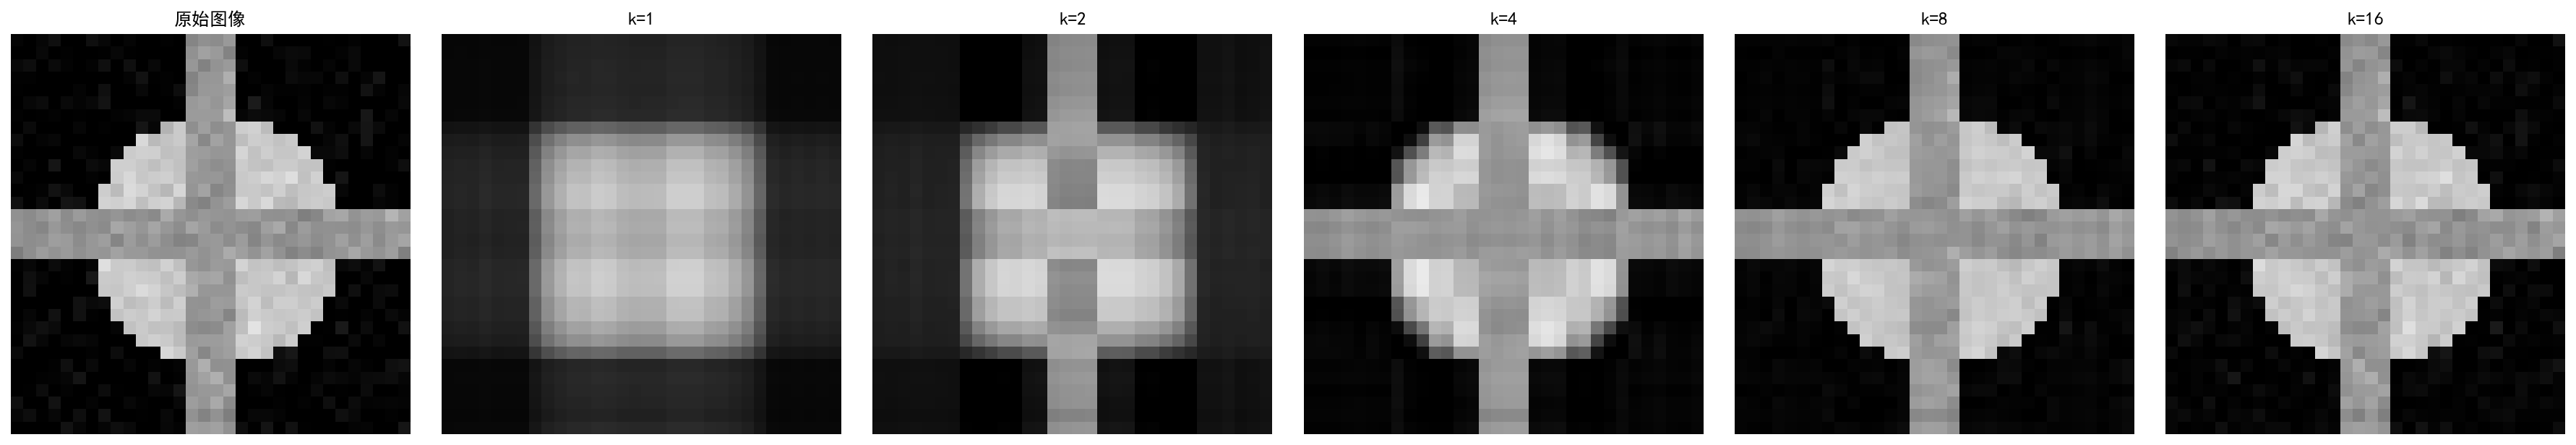
\includegraphics[width=0.9\textwidth]{compression_comparison.png}
    \caption{不同$k$值的SVD压缩效果对比}
    \label{fig:comparison}
\end{figure}

从图中可以看出：
\begin{itemize}
    \item $k=1$ 时，图像严重失真，仅保留基本亮度信息
    \item $k=4$ 时，图像轮廓已基本可辨识
    \item $k=8$ 时，图像质量显著提升，细节较为清晰
    \item $k=16$ 时，图像与原图几乎无法区分
\end{itemize}

\subsection{奇异值分布}

图\ref{fig:svd}展示了奇异值的分布情况及累积能量曲线。

\begin{figure}[H]
    \centering
    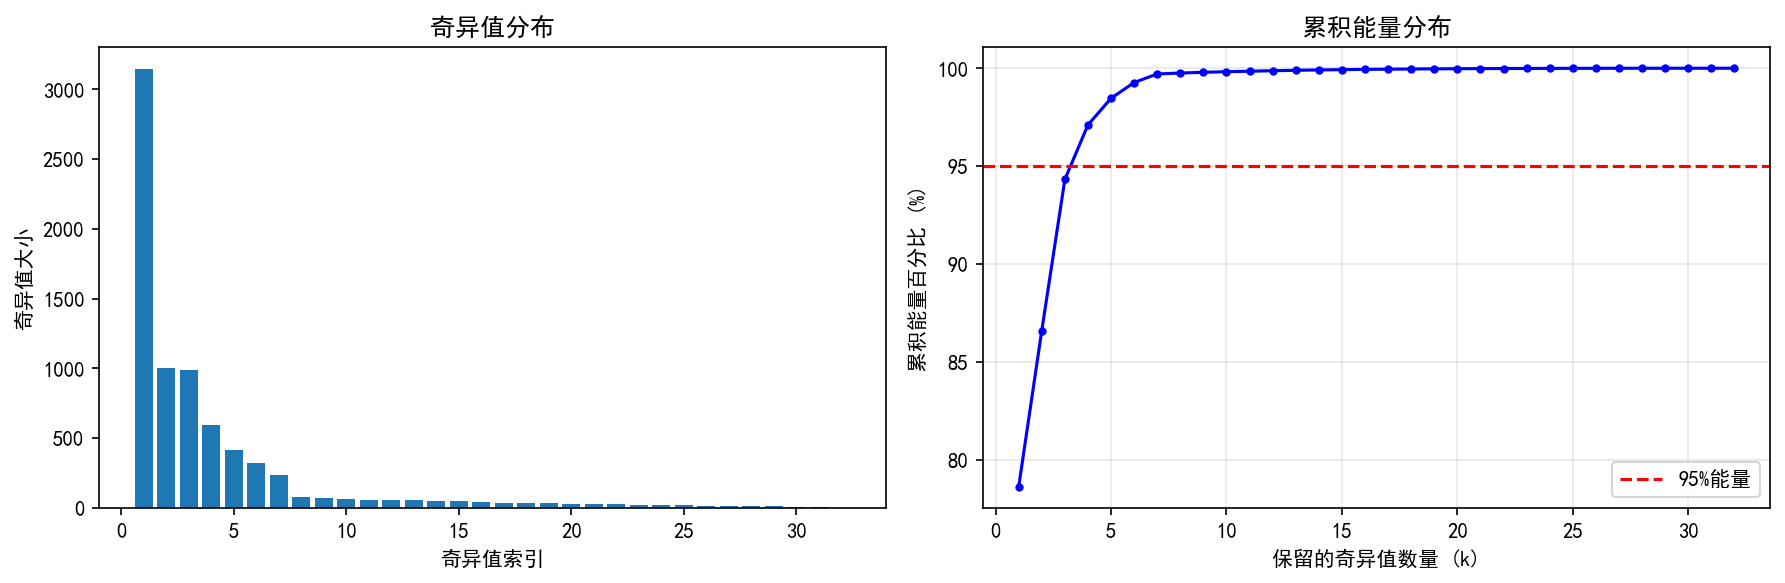
\includegraphics[width=0.9\textwidth]{singular_values.png}
    \caption{奇异值分布与累积能量}
    \label{fig:svd}
\end{figure}

奇异值呈现快速衰减的特征，前几个奇异值占据了图像的大部分能量。这正是SVD压缩有效的根本原因——图像的主要信息集中在少数几个大的奇异值上。

\subsection{误差分析}

表\ref{tab:results}列出了不同 $k$ 值下的定量评价结果。

\begin{table}[H]
\centering
\caption{不同$k$值的压缩性能指标}
\label{tab:results}
\begin{tabular}{@{}ccccc@{}}
\toprule
$k$ & MSE & RMSE & PSNR (dB) & 压缩比 \\
\midrule
1 & 2626.33 & 51.25 & 13.94 & 15.75$\times$ \\
2 & 1646.17 & 40.57 & 15.97 & 7.88$\times$ \\
4 & 355.73 & 18.86 & 22.62 & 3.94$\times$ \\
8 & 30.15 & 5.49 & 33.34 & 1.97$\times$ \\
16 & 7.17 & 2.68 & 39.58 & 0.98$\times$ \\
\bottomrule
\end{tabular}
\end{table}

图\ref{fig:error}展示了误差指标与压缩比的关系。

\begin{figure}[H]
    \centering
    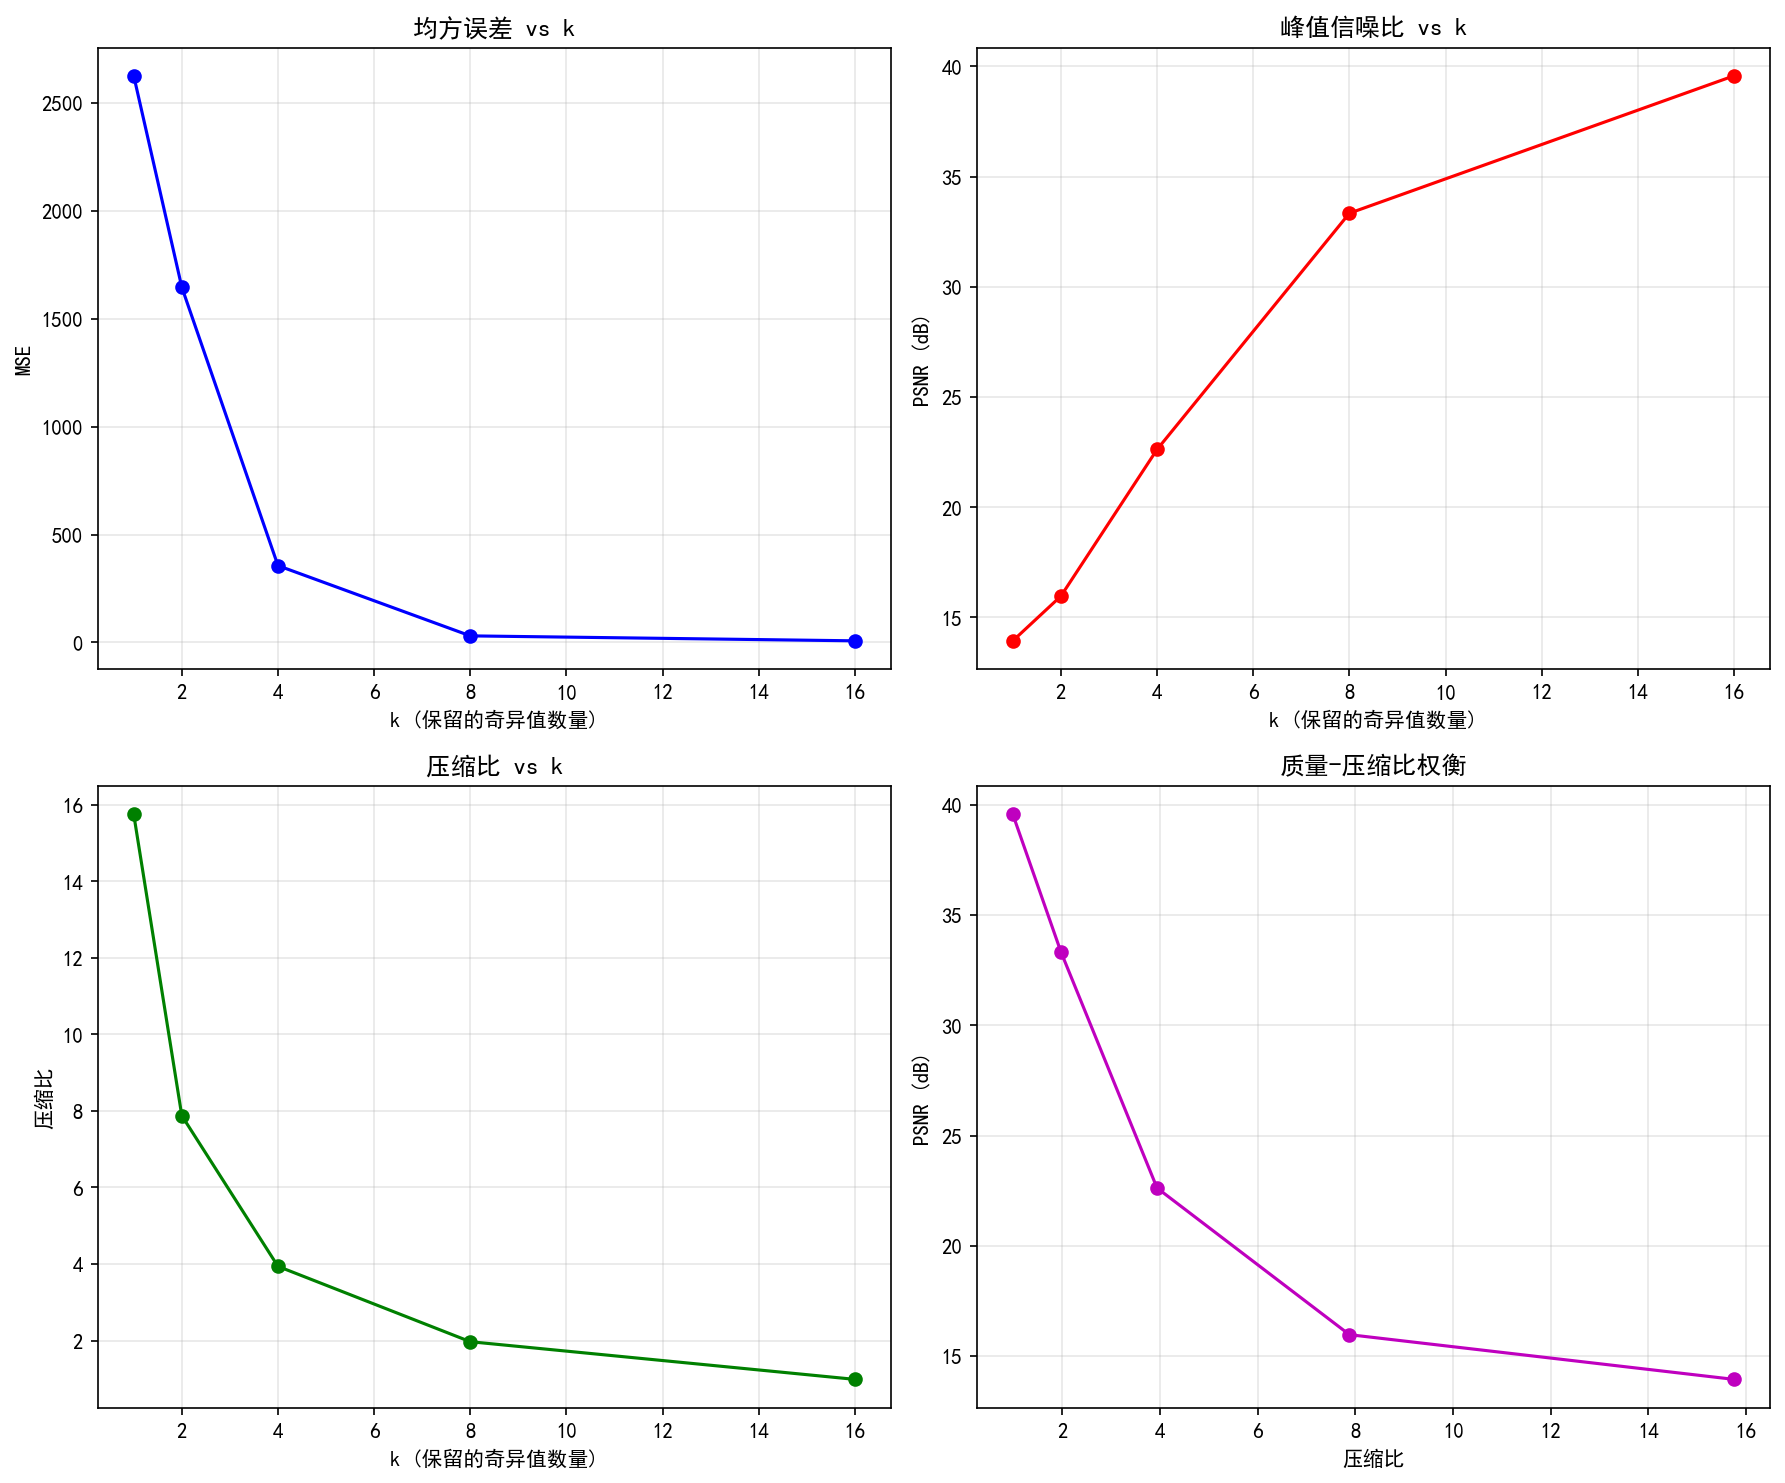
\includegraphics[width=0.9\textwidth]{error_analysis.png}
    \caption{误差分析：MSE、PSNR与压缩比的关系}
    \label{fig:error}
\end{figure}

\subsection{结果讨论}

实验结果表明：

\begin{enumerate}
    \item \textbf{压缩效率：} 当 $k=8$ 时，压缩比约为2倍，PSNR达到33.34 dB，已超过一般认为的30 dB质量阈值，表明SVD压缩在较低压缩比下即可获得良好的视觉效果。
    
    \item \textbf{质量-压缩比权衡：} 随着 $k$ 增大，图像质量提升但压缩比下降。实际应用中需根据具体需求选择合适的 $k$ 值。
    
    \item \textbf{能量集中性：} 奇异值的快速衰减特性使得少量奇异值即可捕获图像的主要信息，这是SVD压缩高效的根本原因。
    
    \item \textbf{渐进性：} SVD压缩具有渐进性——可以通过增加 $k$ 值逐步提升图像质量，这一特性在图像传输中非常有用。
\end{enumerate}

\section{结论}

\subsection{主要贡献}

本文系统研究了SVD的理论基础、几何意义及其在图像压缩中的应用。主要贡献包括：

\begin{enumerate}
    \item 从数学和几何两个角度阐释了SVD定理，揭示了"旋转-缩放-旋转"的变换本质
    \item 提出了基于SVD的图像压缩实现方案，并进行了详细的误差分析
    \item 通过实验验证了SVD压缩的有效性，为实际应用提供了参考依据
\end{enumerate}

\subsection{局限性}

本文研究存在以下局限性：

\begin{enumerate}
    \item 实验图像较小（$32 \times 32$），未在大规模图像上验证
    \item 仅考虑了灰度图像，未涉及彩色图像压缩
    \item 未与其他压缩算法（如JPEG）进行对比分析
\end{enumerate}

\subsection{未来研究方向}

未来研究可从以下方向展开：

\begin{enumerate}
    \item 将SVD压缩扩展到彩色图像（对RGB三个通道分别处理）
    \item 研究分块SVD压缩策略，提升对大图像的压缩效果
    \item 结合深度学习方法，探索自适应的奇异值选择策略
    \item 将SVD与其他压缩算法结合，设计混合压缩方案
\end{enumerate}

\section*{参考文献}

\begin{thebibliography}{99}

\bibitem{strang}
Strang, G. (2016). \textit{Introduction to Linear Algebra} (5th ed.). Wellesley-Cambridge Press.

\bibitem{golub}
Golub, G. H., \& Van Loan, C. F. (2013). \textit{Matrix Computations} (4th ed.). Johns Hopkins University Press.

\bibitem{kalman}
Kalman, D. (1996). A singularly valuable decomposition: The SVD of a matrix. \textit{The College Mathematics Journal}, 27(1), 2-23.

\bibitem{image}
Gonzalez, R. C., \& Woods, R. E. (2018). \textit{Digital Image Processing} (4th ed.). Pearson.

\bibitem{compression}
Sayood, K. (2017). \textit{Introduction to Data Compression} (5th ed.). Morgan Kaufmann.

\end{thebibliography}

\end{document}